% ============================================================
% DESARROLLO - Diseño de Filtros Digitales IIR
% ============================================================

Los parámetros del sistema son:

\begin{itemize}
    \item \textbf{Frecuencia de muestreo:} $f_s = 8000$ Hz
    \item \textbf{Período de muestreo:} $T = \dfrac{1}{f_s} = \dfrac{1}{8000} = 1.25 \times 10^{-4}$ s $= 125\;\mu$s
    \item \textbf{Frecuencia de Nyquist:} $f_N = \dfrac{f_s}{2} = 4000$ Hz
    \item \textbf{Entrada analógica:} GP26 (ADC0)
    \item \textbf{Generación de señal de prueba:} GP3 (PWM, onda cuadrada)
\end{itemize}

Para el uso de los hilos en la pico: el \textbf{Núcleo 1} ejecuta la ecuación en diferencias del filtro 
activo con temporización precisa a $f_s = 8000$ Hz, mientras que el \textbf{Núcleo 0} 
procesa todas las entradas que se van recibiendo.

% ============================================================
\subsection{Filtro Pasa Bajas de Primer Orden (IIR Butterworth)}
% ============================================================


Se selecciona una frecuencia de corte $f_c = 500$ Hz para el filtro pasa bajas. 
Esto por:

\begin{enumerate}
    \item \textbf{Criterio de Nyquist:} La frecuencia de corte debe satisfacer $f_c < f_N = 4000$ Hz, con $f_c = 500$ Hz.

    \item \textbf{Relación $f_c/f_s$:} La relación $f_c/f_s = 500/8000 = 0.0625$ se encuentra en el rango de 
    $(0.01 < f_c/f_s < 0.45)$, lo que hace que la transformada bilineal no introduzca distorsión por efecto de frequency warping.

\end{enumerate}

\textbf{Circuito eléctrico}

El filtro pasa bajas analógico de primer orden se implementa con un circuito RC serie, donde la salida se toma sobre el capacitor:

\begin{figure}[H]
    \centering
    \begin{circuitikz}[american, scale=1.0]
        \draw (0,0) to[V, v=$V_{in}$] (0,3)
              to[R, l=$R$, i>=$i(t)$] (4,3)
              -- (4,3)
              to[C, l_=$C$, v^=$V_{out}$] (4,0)
              -- (0,0);
        \draw (4,3) to[short, -o] (5.5,3);
        \draw (4,0) to[short, -o] (5.5,0);
        \node[right] at (5.5,3) {$+$};
        \node[right] at (5.5,0) {$-$};
    \end{circuitikz}
    \caption{Circuito RC pasa bajas de primer orden.}
    \label{fig:rc_lowpass}
\end{figure}

\textbf{calculo de componentes:}

La frecuencia de corte del circuito RC está dada por:
\begin{equation}
    f_c = \frac{1}{2\pi RC} \quad \Longrightarrow \quad \omega_c = \frac{1}{RC} = 2\pi f_c
\end{equation}

Seleccionando $C = 100$ nF (serie E24), se calcula la resistencia necesaria para obtener $f_c = 500$ Hz:
\begin{equation}
    R = \frac{1}{2\pi f_c C} = \frac{1}{2\pi (500)(100 \times 10^{-9})} = \frac{1}{3.14159 \times 10^{-4}} = 3183.1\;\Omega \approx 3.18\;\text{k}\Omega
\end{equation}

Se utiliza una resistencia de $R = 3.3\;\text{k}\Omega$ (serie E24), lo cual resulta en una frecuencia de corte real de:
\begin{equation}
    f_{c,\text{real}} = \frac{1}{2\pi (3300)(100 \times 10^{-9})} = \frac{1}{2.0735 \times 10^{-3}} = 482.3\;\text{Hz}
\end{equation}

Esta desviación de $\approx 3.5\%$ respecto al valor teórico es aceptable.

\subsubsection{Obtención de la función de transferencia $H(s)$}

Aplicando la ley de Kirchhoff al circuito RC en el dominio de Laplace:
\begin{equation}
    V_{in}(s) = R \cdot I(s) + \frac{1}{sC} \cdot I(s) = I(s)\left(R + \frac{1}{sC}\right)
\end{equation}

El voltaje de salida sobre el capacitor es:
\begin{equation}
    V_{out}(s) = \frac{1}{sC} \cdot I(s)
\end{equation}

Despejando la corriente de la primera ecuación y sustituyendo:
\begin{equation}
    H(s) = \frac{V_{out}(s)}{V_{in}(s)} = \frac{\dfrac{1}{sC}}{R + \dfrac{1}{sC}} = \frac{1}{sRC + 1}
\end{equation}

Multiplicando numerador y denominador por $\omega_c = 1/(RC)$:
\begin{equation}
    \boxed{H(s) = \frac{\omega_c}{s + \omega_c}, \qquad \omega_c = 2\pi(500) = 3141.59\;\text{rad/s}}
    \label{eq:lp_hs}
\end{equation}

Esta es la función de transferencia de un filtro Butterworth pasa bajas de primer orden, con ganancia unitaria en DC ($H(0)=1$) y atenuación de $-3$ dB en $\omega = \omega_c$.

\subsubsection{Discretización mediante la transformada bilineal}

\paragraph{Paso 1: Pre-distorsión de frecuencia.}

La transformada bilineal introduce una distorsión no lineal entre las frecuencias analógica y digital. 
Para garantizar que la frecuencia de corte sea exactamente la misma y se mantenga, 
se calcula la frecuencia analógica pre-distorsionada:
\begin{equation}
    \Omega_a = \tan\left(\frac{\pi f_c}{f_s}\right) = \tan\left(\frac{\pi \cdot 500}{8000}\right) = \tan\left(\frac{\pi}{16}\right)
\end{equation}

Evaluando:
\begin{equation}
    \Omega_a = \tan(0.19635\;\text{rad}) = 0.19891
    \label{eq:omega_a_lp}
\end{equation}


\begin{equation}
    H(s) = \frac{\Omega_a}{s + \Omega_a}
\end{equation}

\paragraph{Paso 2: Sustitución de la variable bilineal.}

\begin{equation}
    s = \frac{z - 1}{z + 1}
\end{equation}

Sustituyendo en $H(s)$:
\begin{equation}
    H(z) = \frac{\Omega_a}{\dfrac{z-1}{z+1} + \Omega_a}
\end{equation}

\textbf{simplificando:}

Multiplicando numerador y denominador por $(z+1)$:
\begin{equation}
    H(z) = \frac{\Omega_a (z + 1)}{(z - 1) + \Omega_a(z + 1)}
\end{equation}

Expandiendo el denominador:
\begin{align}
    (z - 1) + \Omega_a(z + 1) &= z - 1 + \Omega_a z + \Omega_a \nonumber \\
    &= z(1 + \Omega_a) + (\Omega_a - 1)
\end{align}

Dividiendo numerador y denominador entre $(1 + \Omega_a)$:
\begin{equation}
    H(z) = \frac{\dfrac{\Omega_a}{1+\Omega_a}\;(z + 1)}{z + \dfrac{\Omega_a - 1}{1 + \Omega_a}} = \frac{\dfrac{\Omega_a}{1+\Omega_a}\;(z + 1)}{z - \dfrac{1 - \Omega_a}{1 + \Omega_a}}
\end{equation}

\paragraph{Paso 3: Identificación con la forma estándar.}

Comparando con la forma canónica $H(z) = \dfrac{A_0 z + A_1}{z - B_1}$:

\begin{align}
    A_0 = A_1 &= \frac{\Omega_a}{1 + \Omega_a} = \frac{0.19891}{1 + 0.19891} = \frac{0.19891}{1.19891} = 0.16591 \\[6pt]
    B_1 &= \frac{1 - \Omega_a}{1 + \Omega_a} = \frac{1 - 0.19891}{1 + 0.19891} = \frac{0.80109}{1.19891} = 0.66818
\end{align}

Por lo tanto, la función de transferencia discreta es:
\begin{equation}
    \boxed{H(z) = \frac{0.16591\;(z + 1)}{z - 0.66818} = \frac{0.16591\,z + 0.16591}{z - 0.66818}}
    \label{eq:lp_hz}
\end{equation}

\subsubsection{Ecuación en diferencias}

A partir de $H(z) = Y(z)/U(z)$:
\begin{equation}
    Y(z)\,(z - B_1) = U(z)\,(A_0\,z + A_1)
\end{equation}

Dividiendo ambos lados entre $z$:
\begin{equation}
    Y(z) - B_1\,z^{-1}\,Y(z) = A_0\,U(z) + A_1\,z^{-1}\,U(z)
\end{equation}

Aplicando la transformada $z$ inversa (donde $z^{-1}$ representa un retardo de una muestra):
\begin{equation}
    \boxed{y(k) = A_0 \cdot u(k) + A_1 \cdot u(k-1) + B_1 \cdot y(k-1)}
    \label{eq:lp_diff}
\end{equation}

Sustituyendo los valores numéricos:
\begin{equation}
    y(k) = 0.16591 \cdot u(k) + 0.16591 \cdot u(k-1) + 0.66818 \cdot y(k-1)
\end{equation}

\textbf{Coeficientes:}

\begin{table}[H]
    \centering
    \caption{Coeficientes del filtro pasa bajas de primer orden ($f_c = 500$ Hz, $f_s = 8000$ Hz).}
    \label{tab:lp_coeff}
    \begin{tabular}{|c|c|c|}
        \hline
        \rowcolor{headblue}\textcolor{white}{\textbf{Coeficiente}} & \textcolor{white}{\textbf{Expresión}} & \textcolor{white}{\textbf{Valor numérico}} \\
        \hline
        $A_0$ & $\dfrac{\Omega_a}{1 + \Omega_a}$ & $0.16591$ \\[10pt]
        \hline
        $A_1$ & $\dfrac{\Omega_a}{1 + \Omega_a}$ & $0.16591$ \\[10pt]
        \hline
        $A_2$ & --- & $0.0$ \\[4pt]
        \hline
        $B_1$ & $\dfrac{1 - \Omega_a}{1 + \Omega_a}$ & $0.66818$ \\[10pt]
        \hline
        $B_2$ & --- & $0.0$ \\[4pt]
        \hline
    \end{tabular}
\end{table}

\textbf{Verificación en DC ($z = 1$):}
\begin{equation}
    H(1) = \frac{A_0 + A_1}{1 - B_1} = \frac{0.16591 + 0.16591}{1 - 0.66818} = \frac{0.33182}{0.33182} = 1.0 
\end{equation}

De este modo, se verifica que la componente DC no sufre atenuación.

\subsubsection{Diagrama de flujo de señal}

\begin{figure}[H]
    \centering
    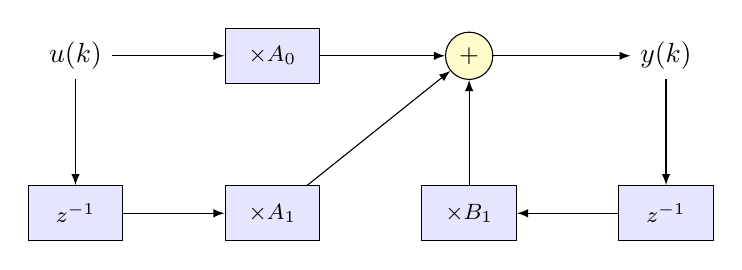
\begin{tikzpicture}[
        block/.style={draw, fill=blue!10, minimum width=1.2cm, minimum height=0.7cm, font=\footnotesize},
        sum/.style={draw, circle, fill=yellow!20, minimum size=0.6cm, inner sep=0pt, font=\small},
        >=latex
    ]
        % Main signal path
        \node (in) at (0,0) {$u(k)$};
        \node[block] (A0) at (2.5,0) {$\times A_0$};
        \node[sum] (S) at (5,0) {$+$};
        \node (out) at (7.5,0) {$y(k)$};

        % u delay line
        \node[block] (Z1) at (0,-2) {$z^{-1}$};
        \node[block] (A1) at (2.5,-2) {$\times A_1$};

        % y feedback
        \node[block] (Z2) at (7.5,-2) {$z^{-1}$};
        \node[block] (B1) at (5,-2) {$\times B_1$};

        % Connections: feedforward
        \draw[->] (in) -- (A0);
        \draw[->] (A0) -- (S);
        \draw[->] (S) -- (out);

        % u delay
        \draw[->] (in) -- (Z1);
        \draw[->] (Z1) -- (A1);
        \draw[->] (A1) -- (S);

        % y feedback
        \draw[->] (out) -- (Z2);
        \draw[->] (Z2) -- (B1);
        \draw[->] (B1) -- (S);
    \end{tikzpicture}
    \caption{Diagrama de flujo de señal del filtro pasa bajas de primer orden (Forma Directa I).}
    \label{fig:lp_signal_flow}
\end{figure}

% ============================================================
\newpage
\subsection{Diseño del Filtro Pasa Altas de Segundo Orden (Circuito RLC)}
% ============================================================

Se selecciona una frecuencia de corte $f_c = 800$ Hz para el filtro pasa altas de segundo orden. 
Para esto, se tomo en cuenta lo siguiente:

\begin{enumerate}
    \item \textbf{Criterio de Nyquist:} Se cumple $f_c = 800\;\text{Hz} < f_N = 4000\;\text{Hz}$.

    \item \textbf{Relación:} La relación $f_c/f_s = 800/8000 = 0.1$ se ubica en la zona central del rango recomendado, donde la transformada bilineal presenta mínima distorsión.

\end{enumerate}

\textbf{Circuito:}

El filtro pasa altas de segundo orden se implementa obligatoriamente con un circuito \textbf{RLC serie}, ya que para obtener una función de transferencia de segundo grado se requieren al menos dos elementos almacenadores (capacitor e inductor).

\begin{figure}[H]
    \centering
    \begin{circuitikz}[american, scale=1.0]
        \draw (0,0) to[V, v=$V_{in}$] (0,3)
              to[C, l=$C$, i>=$i(t)$] (3,3)
              to[R, l=$R$] (6,3)
              to[L, l=$L$] (6,0)
              -- (0,0);
        \draw (6,3) to[short, -o] (7.8,3);
        \draw (6,0) to[short, -o] (7.8,0);
        \node[right] at (7.8,3) {$+$};
        \node[right] at (7.8,0) {$-$};
        \node[right] at (7.8,1.5) {$V_{out}$};
    \end{circuitikz}
    \caption{Circuito RLC serie pasa altas de segundo orden (salida sobre el inductor $L$).}
    \label{fig:rlc_highpass}
\end{figure}

\textbf{calculo de los componentes:}

Del circuito RLC serie se obtiene:

\begin{equation}
    H(s) = \frac{s^2}{s^2 + \dfrac{R}{L}\,s + \dfrac{1}{LC}}
\end{equation}

Comparando con la forma canónica Butterworth de segundo orden:
\begin{equation}
    H(s) = \frac{s^2}{s^2 + \sqrt{2}\,\omega_c\,s + \omega_c^2}
\end{equation}

Se identifican las relaciones de diseño:
\begin{equation}
    \frac{1}{LC} = \omega_c^2, \qquad \frac{R}{L} = \sqrt{2}\,\omega_c
    \label{eq:rlc_relations}
\end{equation}

Con $\omega_c = 2\pi(800) = 5026.55$ rad/s y $L = 100$ mH:

\begin{align}
    C &= \frac{1}{L \cdot \omega_c^2} = \frac{1}{0.1 \times (5026.55)^2} = \frac{1}{0.1 \times 25{,}266{,}219} = \frac{1}{2{,}526{,}622} \nonumber \\[6pt]
    C &= 3.958 \times 10^{-7}\;\text{F} = 395.8\;\text{nF} \approx 390\;\text{nF}\;
\end{align}

\begin{align}
    R &= \sqrt{2}\,\omega_c \cdot L = 1.41421 \times 5026.55 \times 0.1 \nonumber \\[6pt]
    R &= 710.8\;\Omega\;
\end{align}


\subsubsection{Obtención de la función de transferencia $H(s)$}

Aplicando la LVK al circuito RLC serie en el dominio de Laplace:
\begin{equation}
    V_{in}(s) = \frac{1}{sC}\,I(s) + R\,I(s) + sL\,I(s) = I(s)\left(\frac{1}{sC} + R + sL\right)
\end{equation}

La salida se toma sobre el inductor:
\begin{equation}
    V_{out}(s) = sL \cdot I(s)
\end{equation}

La función de transferencia es:
\begin{equation}
    H(s) = \frac{V_{out}(s)}{V_{in}(s)} = \frac{sL}{\dfrac{1}{sC} + R + sL}
\end{equation}

Multiplicando numerador y denominador por $sC$:
\begin{equation}
    H(s) = \frac{s^2 LC}{s^2 LC + sRC + 1}
\end{equation}

Dividiendo entre $LC$:
\begin{equation}
    \boxed{H(s) = \frac{s^2}{s^2 + \dfrac{R}{L}\,s + \dfrac{1}{LC}} = \frac{s^2}{s^2 + \sqrt{2}\,\omega_c\,s + \omega_c^2}}
    \label{eq:hp_hs}
\end{equation}

donde $\omega_c = 2\pi(800) = 5026.55$ rad/s. La ganancia es cero en DC ($H(0)=0$, bloquea la componente continua) y unitaria en alta frecuencia ($\lim_{s\to\infty}H(s)=1$), confirmando el comportamiento pasa altas.

\subsubsection{Discretización mediante la transformada bilineal (Tustin)}

\paragraph{Paso 1: Pre-distorsión de frecuencia.}

\begin{equation}
    \Omega_a = \tan\left(\frac{\pi f_c}{f_s}\right) = \tan\left(\frac{\pi \cdot 800}{8000}\right) = \tan\left(\frac{\pi}{10}\right) = \tan(18°) = 0.32492
    \label{eq:omega_a_hp}
\end{equation}

\begin{equation}
    H(s) = \frac{s^2}{s^2 + \sqrt{2}\,\Omega_a\,s + \Omega_a^2}
\end{equation}

\paragraph{Paso 2: Sustitución bilineal $s = \dfrac{z-1}{z+1}$.}

\begin{equation}
    H(z) = \frac{\left(\dfrac{z-1}{z+1}\right)^2}{\left(\dfrac{z-1}{z+1}\right)^2 + \sqrt{2}\,\Omega_a\left(\dfrac{z-1}{z+1}\right) + \Omega_a^2}
\end{equation}

\textbf{Simplificacion:}

Multiplicando numerador y denominador por $(z+1)^2$:
\begin{equation}
    H(z) = \frac{(z-1)^2}{(z-1)^2 + \sqrt{2}\,\Omega_a\,(z-1)(z+1) + \Omega_a^2\,(z+1)^2}
\end{equation}

Expandiendo cada término del denominador por separado:
\begin{align}
    (z-1)^2 &= z^2 - 2z + 1 \\[4pt]
    \sqrt{2}\,\Omega_a\,(z-1)(z+1) &= \sqrt{2}\,\Omega_a\,(z^2 - 1) = 0.45944\,z^2 - 0.45944 \\[4pt]
    \Omega_a^2\,(z+1)^2 &= 0.10557\,(z^2 + 2z + 1) = 0.10557\,z^2 + 0.21114\,z + 0.10557
\end{align}

Agrupando el denominador por potencias:
\begin{equation}
    D(z) = z^2\underbrace{(1 + 0.45944 + 0.10557)}_{D_0} + z\underbrace{(-2 + 0 + 0.21114)}_{D_1} + \underbrace{(1 - 0.45944 + 0.10557)}_{D_2}
\end{equation}

Evaluando:
\begin{align}
    D_0 &= 1 + \sqrt{2}\,\Omega_a + \Omega_a^2 = 1 + 0.45944 + 0.10557 = 1.56501 \\[4pt]
    D_1 &= -2 + 2\Omega_a^2 = -2 + 2(0.10557) = -2 + 0.21114 = -1.78886 \\[4pt]
    D_2 &= 1 - \sqrt{2}\,\Omega_a + \Omega_a^2 = 1 - 0.45944 + 0.10557 = 0.64613
\end{align}

\paragraph{Paso 4: Normalizando:}

Dividiendo numerador y denominador entre $D_0 = 1.56501$:

\begin{equation}
    H(z) = \frac{\dfrac{1}{D_0}\,(z^2 - 2z + 1)}{z^2 + \dfrac{D_1}{D_0}\,z + \dfrac{D_2}{D_0}}
\end{equation}

Calculando cada coeficiente:
\begin{align}
    A_0 &= \frac{1}{D_0} = \frac{1}{1.56501} = 0.63897 \\[6pt]
    A_1 &= \frac{-2}{D_0} = \frac{-2}{1.56501} = -1.27795 \\[6pt]
    A_2 &= \frac{1}{D_0} = \frac{1}{1.56501} = 0.63897
\end{align}

Para los coeficientes del denominador, se utiliza la convención de la ecuación en diferencias $y(k) = \cdots + B_1\,y(k-1) + B_2\,y(k-2)$:
\begin{align}
    B_1 &= -\frac{D_1}{D_0} = -\frac{-1.78886}{1.56501} = 1.14305 \\[6pt]
    B_2 &= -\frac{D_2}{D_0} = -\frac{0.64613}{1.56501} = -0.41286
\end{align}

La función de transferencia discreta resulta:
\begin{equation}
    \boxed{H(z) = \frac{0.63897\,z^2 - 1.27795\,z + 0.63897}{z^2 - 1.14305\,z + 0.41286}}
    \label{eq:hp_hz}
\end{equation}

\subsubsection{Ecuación en diferencias}

A partir de $H(z) = Y(z)/U(z)$:
\begin{equation}
    Y(z)\,(z^2 - B_1\,z - B_2) = U(z)\,(A_0\,z^2 + A_1\,z + A_2)
\end{equation}

Dividiendo ambos lados entre $z^2$ y aplicando la transformada $z$ inversa:
\begin{equation}
    y(k) - B_1\,y(k-1) - B_2\,y(k-2) = A_0\,u(k) + A_1\,u(k-1) + A_2\,u(k-2)
\end{equation}

Reorganizando:
\begin{equation}
    \boxed{y(k) = A_0\,u(k) + A_1\,u(k-1) + A_2\,u(k-2) + B_1\,y(k-1) + B_2\,y(k-2)}
    \label{eq:hp_diff}
\end{equation}

Sustituyendo los valores numéricos:
\begin{multline}
    y(k) = 0.63897\,u(k) - 1.27795\,u(k-1) + 0.63897\,u(k-2) \\
    + 1.14305\,y(k-1) - 0.41286\,y(k-2)
\end{multline}

\textbf{coeficientes:}

\begin{table}[H]
    \centering
    \caption{Coeficientes del filtro pasa altas de segundo orden ($f_c = 800$ Hz, $f_s = 8000$ Hz).}
    \label{tab:hp_coeff}
    \begin{tabular}{|c|c|c|}
        \hline
        \rowcolor{headblue}\textcolor{white}{\textbf{Coeficiente}} & \textcolor{white}{\textbf{Expresión}} & \textcolor{white}{\textbf{Valor numérico}} \\
        \hline
        $A_0$ & $\dfrac{1}{D_0}$ & $0.63897$ \\[10pt]
        \hline
        $A_1$ & $\dfrac{-2}{D_0}$ & $-1.27795$ \\[10pt]
        \hline
        $A_2$ & $\dfrac{1}{D_0}$ & $0.63897$ \\[10pt]
        \hline
        $B_1$ & $-\dfrac{D_1}{D_0}$ & $1.14305$ \\[10pt]
        \hline
        $B_2$ & $-\dfrac{D_2}{D_0}$ & $-0.41286$ \\[10pt]
        \hline
    \end{tabular}
\end{table}

\newpage

\begin{enumerate}
    \item \textbf{En DC ($z = 1$):}
    \begin{equation}
        H(1) = \frac{A_0 + A_1 + A_2}{1 - B_1 - B_2} = \frac{0.63897 - 1.27795 + 0.63897}{1 - 1.14305 + 0.41286} = \frac{0}{0.26981} = 0 
    \end{equation}
    Esto confirma que el filtro pasa altas bloquea completamente la componente DC.

    \item \textbf{En Nyquist ($z = -1$):}
    \begin{equation}
        H(-1) = \frac{A_0 - A_1 + A_2}{1 + B_1 - B_2} = \frac{0.63897 + 1.27795 + 0.63897}{1 + 1.14305 + 0.41286} = \frac{2.55589}{2.55591} \approx 1.0 
    \end{equation}
    Esto confirma que la ganancia es unitaria en la frecuencia de Nyquist.

    \item \textbf{Suma de coeficientes del numerador:}
    \begin{equation}
        A_0 + A_1 + A_2 = 0.63897 - 1.27795 + 0.63897 = 0
    \end{equation}
    garantiza $H(1)=0$.
\end{enumerate}

\subsubsection{Diagrama de flujo de señal}

\begin{figure}[H]
    \centering
    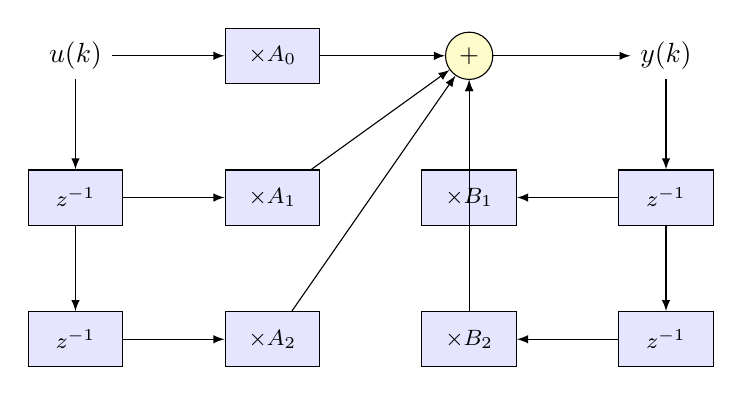
\begin{tikzpicture}[
        block/.style={draw, fill=blue!10, minimum width=1.2cm, minimum height=0.7cm, font=\footnotesize},
        sum/.style={draw, circle, fill=yellow!20, minimum size=0.6cm, inner sep=0pt, font=\small},
        >=latex
    ]
        % Main signal path
        \node (in) at (0,0) {$u(k)$};
        \node[block] (A0) at (2.5,0) {$\times A_0$};
        \node[sum] (S) at (5,0) {$+$};
        \node (out) at (7.5,0) {$y(k)$};

        % Input delay chain
        \node[block] (Z1u) at (0,-1.8) {$z^{-1}$};
        \node[block] (A1) at (2.5,-1.8) {$\times A_1$};
        \node[block] (Z2u) at (0,-3.6) {$z^{-1}$};
        \node[block] (A2) at (2.5,-3.6) {$\times A_2$};

        % Output delay chain (feedback)
        \node[block] (Z1y) at (7.5,-1.8) {$z^{-1}$};
        \node[block] (B1) at (5,-1.8) {$\times B_1$};
        \node[block] (Z2y) at (7.5,-3.6) {$z^{-1}$};
        \node[block] (B2) at (5,-3.6) {$\times B_2$};

        % Feedforward connections
        \draw[->] (in) -- (A0);
        \draw[->] (A0) -- (S);
        \draw[->] (S) -- (out);

        % Input delays
        \draw[->] (in) -- (Z1u);
        \draw[->] (Z1u) -- (A1);
        \draw[->] (A1) -- (S);
        \draw[->] (Z1u) -- (Z2u);
        \draw[->] (Z2u) -- (A2);
        \draw[->] (A2) -- (S);

        % Feedback delays
        \draw[->] (out) -- (Z1y);
        \draw[->] (Z1y) -- (B1);
        \draw[->] (B1) -- (S);
        \draw[->] (Z1y) -- (Z2y);
        \draw[->] (Z2y) -- (B2);
        \draw[->] (B2) -- (S);
    \end{tikzpicture}
    \caption{Diagrama de flujo de señal del filtro pasa altas de segundo orden (Forma Directa I).}
    \label{fig:hp_signal_flow}
\end{figure}



% ============================================================
\newpage
\subsection{Implementación en MicroPython}
% ============================================================

\subsubsection{Documentación del código}

El programa comienza importando las bibliotecas necesarias para interactuar con el hardware de la Raspberry Pi Pico 2W. De la biblioteca \texttt{machine} se traen las clases \texttt{Pin}, \texttt{ADC} y \texttt{PWM}, que permiten configurar pines digitales, leer señales analógicas y generar ondas con modulación de ancho de pulso, respectivamente. También se importa el módulo \texttt{\_thread}, que es la herramienta que ofrece MicroPython para trabajar con los dos núcleos del procesador RP2350 de forma simultánea, y el módulo \texttt{time}, que se utiliza para medir tiempos y hacer pausas con precisión de microsegundos. Además se importan \texttt{sys} y \texttt{select}, necesarios para implementar la lectura del puerto serial de forma no bloqueante.

A continuación se definen los parámetros fundamentales del sistema. La frecuencia de muestreo se fija en 8000~Hz, lo que implica que el filtro debe calcular una nueva muestra cada 125~microsegundos. Estos valores se guardan en las constantes \texttt{FS} y \texttt{PERIOD\_US} para que sean fáciles de modificar si en algún momento se quisiera cambiar la tasa de muestreo. También se define la constante \texttt{PRINT\_SKIP}, que indica cada cuántas muestras se envían datos al puerto serial para su visualización; esto es necesario porque imprimir cada una de las 8000 muestras por segundo desbordaría el buffer USB y provocaría que los comandos dejaran de responder.

Después viene la configuración del hardware. El pin GP26 se configura como entrada analógica a través de la clase \texttt{ADC}, ya que es uno de los pines que tiene convertidor analógico-digital integrado en la Pico. El pin GP3 se configura como salida PWM para generar la onda cuadrada que sirve como señal de prueba; se le asigna una frecuencia inicial de 200~Hz y un ciclo de trabajo del 50\%, lo que produce una onda simétrica. Finalmente, el LED integrado de la placa se configura como salida digital para servir como indicador visual de que el sistema se encuentra filtrando activamente.

Los coeficientes de los dos filtros se declaran como constantes globales. Para el filtro pasa bajas de primer orden, que se diseñó a partir del circuito RC con frecuencia de corte de 500~Hz, los coeficientes son $A_0 = A_1 = 0.16591$ y $B_1 = 0.66818$, obtenidos mediante la transformada bilineal como se mostró en la sección anterior. Para el filtro pasa altas de segundo orden, derivado del circuito RLC con frecuencia de corte de 800~Hz, los coeficientes son $A_0 = 0.63897$, $A_1 = -1.27795$, $A_2 = 0.63897$, $B_1 = 1.14305$ y $B_2 = -0.41286$. Estos valores se almacenan con cinco decimales para mantener una precisión adecuada en los cálculos de punto flotante.

El estado compartido entre los dos núcleos se almacena en una lista mutable de Python llamada \texttt{st}, que contiene once elementos: dos banderas de control (si el filtro está corriendo y cuál filtro está activo), las variables de estado de ambos filtros (entradas y salidas anteriores), y tres valores para la comunicación con el Núcleo~0 (la última entrada leída, la última salida calculada, y una bandera que indica si hay datos nuevos listos para imprimir). Se eligió una lista mutable porque en el RP2350, el Núcleo~1 no puede acceder de manera confiable a las variables globales del módulo principal; al pasar la lista como argumento a la función del hilo, ambos núcleos pueden leer y escribir los mismos datos sin problema, ya que la lista se pasa por referencia. Para hacer el código más legible, se definen constantes con los nombres de cada índice de la lista.

La parte central del programa es la función \texttt{filter\_core}, que se ejecuta en el Núcleo~1 del procesador. Esta función recibe como argumentos todo lo que necesita para operar: la lista de estado compartido, el objeto del ADC, el módulo de tiempo, todos los coeficientes de ambos filtros, el periodo de muestreo y el valor de salto de impresión. De esta forma, la función no hace ninguna referencia a nombres globales del módulo, lo que evita el error de visibilidad que tiene el RP2350 con los hilos. Dentro de un ciclo infinito, mientras la bandera de ejecución esté activa, la función registra el tiempo de inicio, lee el valor del ADC convirtiéndolo a voltaje entre 0 y 3.3~V, y evalúa la ecuación en diferencias del filtro seleccionado. Cada cierto número de muestras (determinado por \texttt{PRINT\_SKIP}), guarda los valores de entrada y salida en la lista compartida y activa la bandera de datos nuevos para que el Núcleo~0 los imprima. Al final de cada iteración, calcula cuánto tiempo tardó el procesamiento y espera el tiempo restante para completar exactamente los 125~microsegundos del periodo de muestreo.

La función \texttt{filter\_core} se lanza en el Núcleo~1 mediante la instrucción \texttt{\_thread.start\_new\_thread}, pasando como argumentos la lista de estado, el objeto del ADC, el módulo de tiempo, los coeficientes de ambos filtros, el periodo y el salto de impresión. De este modo, ambos núcleos del RP2350 trabajan de manera simultánea sin interferirse: el Núcleo~1 se dedica exclusivamente al cálculo del filtro, y nunca accede al puerto serial.

El Núcleo~0 se encarga de toda la comunicación serial. Para poder recibir comandos y al mismo tiempo enviar los datos del filtro al Serial Plotter, se utiliza el mecanismo de \texttt{select.poll()}, que permite verificar si hay datos disponibles en la entrada estándar sin quedarse bloqueado esperando. El ciclo principal del Núcleo~0 hace tres cosas en cada iteración: primero revisa si llegó algún carácter por el puerto serial y, si es así, lo agrega a un buffer hasta recibir un salto de línea, momento en que procesa el comando completo; después revisa si la bandera de datos nuevos está activa en la lista compartida y, si lo está, imprime los valores de entrada y salida en el formato \texttt{entrada,salida} que espera el Serial Plotter; y por último hace una pausa breve de 200~microsegundos antes de repetir. Los comandos disponibles son: \texttt{START} activa el filtrado y enciende el LED; \texttt{STOP} lo detiene, apaga el LED, reinicia las variables de estado del filtro activo y vuelve a mostrar el menú; \texttt{LP} selecciona el filtro pasa bajas y reinicia sus variables; \texttt{HP} hace lo mismo para el filtro pasa altas; \texttt{FREQ} seguido de un número cambia la frecuencia de la onda cuadrada de prueba; y \texttt{STATUS} muestra en pantalla qué filtro está seleccionado, si está activo o detenido, y las frecuencias del sistema y de la onda de prueba.

\subsubsection{Código fuente}

\lstinputlisting[
    language={[LAB]Python},
    caption={Código MicroPython del sistema de filtros digitales IIR para Raspberry Pi Pico 2W.},
    label={lst:filtros_code}
]{code/filtros_iir.py}

\subsubsection{Diagrama de conexión física}

Para probar el sistema, la señal de prueba generada por el pin GP3 (PWM) se conecta directamente al pin GP26 (ADC0) mediante un cable puente. De esta forma, la onda cuadrada producida por el propio microcontrolador entra al convertidor analógico-digital sin necesidad de componentes externos, lo que permite verificar el funcionamiento de los filtros digitales de manera sencilla.

\begin{figure}[H]
    \centering
    \begin{tikzpicture}[scale=1.0]
        \picoboard

        % Cable puente de GP3 (P5) a GP26_A0 (P31)
        \draw[blue, thick, rounded corners=8pt]
            (P5) -- (-1.5, -2.25)
            -- (-1.5, -5.5)
            -- (5.5, -5.5)
            -- (5.5, -4.5)
            -- (P31);

        % Etiquetas del cable
        \node[left, font=\footnotesize\sffamily, blue] at (-1.5, -3.8) {Cable puente};

        % Anotaciones de los pines
        \node[left, font=\scriptsize\sffamily, fill=white, inner sep=1pt] at (-0.8, -2.25) {GP3 (PWM)};
        \node[right, font=\scriptsize\sffamily, fill=white, inner sep=1pt] at (4.8, -4.5) {GP26 (ADC0)};
    \end{tikzpicture}
    \caption{Conexión física: cable puente entre GP3 (salida PWM) y GP26 (entrada ADC) en la Raspberry Pi Pico 2W.}
    \label{fig:conexion_pico}
\end{figure}
